%!TEX root = SysSpec_ClockPendulumAnalyzer.tex
\subsection{Klassendiagramm}
Die Klassen der Software arbeiten nach dem folgenden Klassendiagramm. Es umfasst eine Implementierung der REST Definition und Klassen für die Datenbankanbindung an SQLite.
\begin{figure}[H]
    \centering
    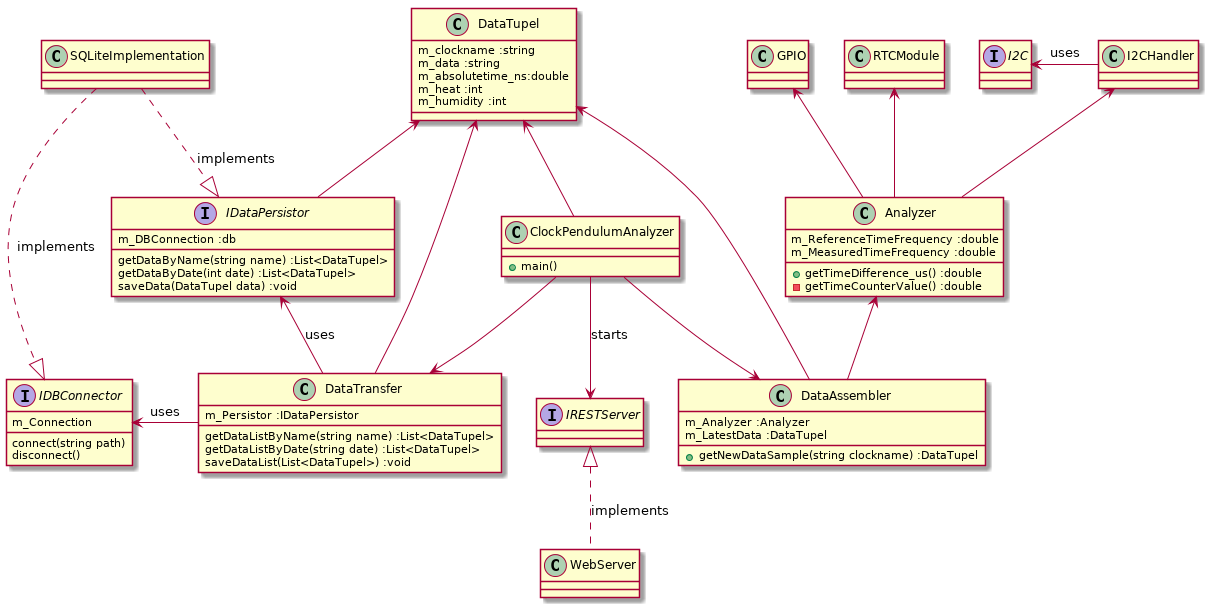
\includegraphics[width=\textwidth]{classdiagramm.png}
    \caption{Klassendiagramm der C++ Software auf dem \rpi}
\end{figure}
\subsubsection{Klassendetails}
    %TODO Klassendiagramm updaten
	\begin{description}
        \item[ClockPendulumAnalyzer] Dies ist die Main Klasse. Sie startet alle Aufgaben.
        \item[I2CHandler] Diese Klasse öffnet und schliesst den $I^2C$-Bus und liest Daten von daran angeschlossenen Geräten.
        \item[GPIO] Eine Klasse die für das Arbeiten mit GPIO Pins auf dem Raspberry Pi zuständig ist.
        \item[Analyzer] Die Klasse ist für die Berechnung der Zeitdifferenz in Nanosekunden zuständig. Es kann auch die Differenz in Mikro- und Millisekunden ausgegeben werden.
        \item[DataAssembler] Die Klasse ist für das Zusammenfügen von Name (aus der Main Klasse) und den einzelnen Dateninputs aus dem Analyzer zuständig. Im Sequenzdiagramm ist dieser Ablauf dargestellt. 
        \item[DataTransfer] Diese Klasse ist für den Transport der DataTupel zwischen Webserver, Mainklasse und Datenbank zuständig.
        \item[DataTupel] Ein Daten Transfer Objekt (DTO) als Abstraktion der gemessenen Daten zu einem gegebenen Zeitpunkt. Beinhaltet Datum+Zeit, Name, Differenz und Werte für Feuchtigkeit und Wärme.
        \item[SQLiteImplementation] Die Implementierung der Schnittstelle \textit{IDataPersistor} und der \textit{IDBConnector} auf eine SQLite Umgebung.
    \end{description}
